% Credits are indicated where needed. The general idea is based on a template by Vel (vel@LaTeXTemplates.com) and Frits Wenneker.

\documentclass[11pt, a4paper]{article} % General settings in the beginning (defines the document class of your paper)
% 11pt = is the font size
% A4 is the paper size
% “article” is your document class

%----------------------------------------------------------------------------------------
%	Packages
%----------------------------------------------------------------------------------------

% Necessary
\usepackage[german,english]{babel} % English and German language 
\usepackage{booktabs} % Horizontal rules in tables 
% For generating tables, use “LaTeX” online generator (https://www.tablesgenerator.com)
\usepackage{comment} % Necessary to comment several paragraphs at once
\usepackage[utf8]{inputenc} % Required for international characters
\usepackage[T1]{fontenc} % Required for output font encoding for international characters

% Might be helpful
\usepackage{amsmath,amsfonts,amsthm} % Math packages which might be useful for equations
\usepackage{tikz} % For tikz figures (to draw arrow diagrams, see a guide how to use them)
\usepackage{tikz-cd}
\usetikzlibrary{positioning,arrows} % Adding libraries for arrows
\usetikzlibrary{decorations.pathreplacing} % Adding libraries for decorations and paths
\usepackage{tikzsymbols} % For amazing symbols ;) https://mirror.hmc.edu/ctan/graphics/pgf/contrib/tikzsymbols/tikzsymbols.pdf 
\usepackage{blindtext} % To add some blind text in your paper
\usepackage[style = alphabetic]{biblatex}
\addbibresource{literature.bib} 

\DeclareMathOperator*{\argmax}{arg\,max}
\usepackage{bbm}
%---------------------------------------------------------------------------------
% Additional settings
%---------------------------------------------------------------------------------

%---------------------------------------------------------------------------------
% Define your margins
\usepackage{geometry} % Necessary package for defining margins

\geometry{
	top=2cm, % Defines top margin
	bottom=2cm, % Defines bottom margin
	left=2.2cm, % Defines left margin
	right=2.2cm, % Defines right margin
	includehead, % Includes space for a header
	%includefoot, % Includes space for a footer
	%showframe, % Uncomment if you want to show how it looks on the page 
}

\setlength{\parindent}{15pt} % Adjust to set you indent globally 

%---------------------------------------------------------------------------------
% Define your spacing
\usepackage{setspace} % Required for spacing
% Two options:
\linespread{1.5}
%\onehalfspacing % one-half-spacing linespread

%----------------------------------------------------------------------------------------
% Define your fonts
\usepackage[T1]{fontenc} % Output font encoding for international characters
\usepackage[utf8]{inputenc} % Required for inputting international characters

\usepackage{XCharter} % Use the XCharter font


%---------------------------------------------------------------------------------
% Define your headers and footers

\usepackage{fancyhdr} % Package is needed to define header and footer
\pagestyle{fancy} % Allows you to customize the headers and footers

%\renewcommand{\sectionmark}[1]{\markboth{#1}{}} % Removes the section number from the header when \leftmark is used

% Headers
\lhead{} % Define left header
\chead{\textit{}} % Define center header - e.g. add your paper title
\rhead{} % Define right header

% Footers
\lfoot{} % Define left footer
\cfoot{\footnotesize \thepage} % Define center footer
\rfoot{ } % Define right footer

%---------------------------------------------------------------------------------
%	Add information on bibliography
%\usepackage{natbib} % Use natbib for citing
%\usepackage{har2nat} % Allows to use harvard package with natbib https://mirror.reismil.ch/CTAN/macros/latex/contrib/har2nat/har2nat.pdf

% For citing with natbib, you may want to use this reference sheet: 
% http://merkel.texture.rocks/Latex/natbib.php

%---------------------------------------------------------------------------------
% Add field for signature (Reference: https://tex.stackexchange.com/questions/35942/how-to-create-a-signature-date-page)
\newcommand{\signature}[2][5cm]{%
  \begin{tabular}{@{}p{#1}@{}}
    #2 \\[2\normalbaselineskip] \hrule \\[0pt]
    {\small \textit{Signature}} \\[2\normalbaselineskip] \hrule \\[0pt]
    {\small \textit{Place, Date}}
  \end{tabular}
}
%---------------------------------------------------------------------------------
%	General information
%---------------------------------------------------------------------------------
\title{Residential Customer Load Pattern Recognition Techniques} % Adds your title
\author{
Lakshya 2017EEB1149 \\ 
Mrityunjay 2017EEB1153 \\ 
Piyush 2017EEB1158 \\ 
Sakib 2017EEB1163 \\ 
Shubham 2017EEB1167 % Add your first and last name
    %\thanks{} % Adds a footnote to your title
    %\institution{YOUR INSTITUTION} % Adds your institution
  }

\date{\small \today} % Adds the current date to your “cover” page; leave empty if you do not want to add a date


%---------------------------------------------------------------------------------
%	Define what’s in your document
%---------------------------------------------------------------------------------

\begin{document}


% If you want a cover page, uncomment "%---------------------------------------------------------------------------------
% Cover page
%---------------------------------------------------------------------------------

% Here are more templates for other cover pages: https://www.latextemplates.com/cat/title-pages

% This example is based on this cover page example: https://www.latextemplates.com/template/academic-title-page

\begin{titlepage} % Starts new environment where the page number is not displayed and the count starts at 1 for the next page

%------------------------------------------------
%	Institutional information
%------------------------------------------------
	
\begin{minipage}{0.4\textwidth} % Begins new environment (like a text box)
    \begin{flushleft} % Sets environment on the left side of the paper
    \large
    University of XX\\ % Add your institution
    Chair of Political Science IV\\ % Add the chair
    Fall 2018\\ % Add term
    COURSE TITLE\\ % Add course title
    Supervisor: NAME % Add instructor/supervisor name 
    \end{flushleft}
\end{minipage}
	
\vspace*{2in} % Adds some space in-between
	
\center % Centre everything on the page

%------------------------------------------------
%	Main part
%------------------------------------------------
	
{\huge\bfseries Residential Customer Load Pattern Recognition Techniques}\\[0.4cm] % Add your paper title 
{\large\today}\\[0.4cm] % Add date (current day)
FIRSTNAME LASTNAME % Add your name
	
\vfill % Adds additional space

%------------------------------------------------
%	General information about the author
%------------------------------------------------

\vfill % Adds additional space

Your contact info \\ % Add your contact info
Your Program \\ % Add info about your program
Semester you are enrolled \\ % Add info about your semester

\vfill % Adds additional space

%------------------------------------------------
%	Word count
%------------------------------------------------

\vfill % Adds additional space
	
Word count: XXXX % To indicate the word count
% How to check words in a LaTeX document: https://www.overleaf.com/help/85-is-there-a-way-to-run-a-word-count-that-doesnt-include-latex-commands
	

	
\end{titlepage}" and uncomment "\begin{comment}" and "\end{comment}" to comment the following lines
%%---------------------------------------------------------------------------------
% Cover page
%---------------------------------------------------------------------------------

% Here are more templates for other cover pages: https://www.latextemplates.com/cat/title-pages

% This example is based on this cover page example: https://www.latextemplates.com/template/academic-title-page

\begin{titlepage} % Starts new environment where the page number is not displayed and the count starts at 1 for the next page

%------------------------------------------------
%	Institutional information
%------------------------------------------------
	
\begin{minipage}{0.4\textwidth} % Begins new environment (like a text box)
    \begin{flushleft} % Sets environment on the left side of the paper
    \large
    University of XX\\ % Add your institution
    Chair of Political Science IV\\ % Add the chair
    Fall 2018\\ % Add term
    COURSE TITLE\\ % Add course title
    Supervisor: NAME % Add instructor/supervisor name 
    \end{flushleft}
\end{minipage}
	
\vspace*{2in} % Adds some space in-between
	
\center % Centre everything on the page

%------------------------------------------------
%	Main part
%------------------------------------------------
	
{\huge\bfseries Residential Customer Load Pattern Recognition Techniques}\\[0.4cm] % Add your paper title 
{\large\today}\\[0.4cm] % Add date (current day)
FIRSTNAME LASTNAME % Add your name
	
\vfill % Adds additional space

%------------------------------------------------
%	General information about the author
%------------------------------------------------

\vfill % Adds additional space

Your contact info \\ % Add your contact info
Your Program \\ % Add info about your program
Semester you are enrolled \\ % Add info about your semester

\vfill % Adds additional space

%------------------------------------------------
%	Word count
%------------------------------------------------

\vfill % Adds additional space
	
Word count: XXXX % To indicate the word count
% How to check words in a LaTeX document: https://www.overleaf.com/help/85-is-there-a-way-to-run-a-word-count-that-doesnt-include-latex-commands
	

	
\end{titlepage}

%\begin{comment}
\maketitle % Print your title, author name and date; comment if you want a cover page 

%\end{comment}

%----------------------------------------------------------------------------------------
% Introduction
%----------------------------------------------------------------------------------------
\setcounter{page}{1} % Sets counter of page to 1

\section{Problem Definition}
Accurate and reliable electric load pattern recognition of residential loads provides critical information that can enable households to effectively manage the electric loads and provides awareness about the actual energy performance of houses. It can also help to estimate the energy consumption of end users, or to detect equipment degradation based on load monitoring system. For example, some electric loads, such as fans, monitors and TVs, could be turned off automatically when not in use. But, the majority of loads connected to a building remain unidentified due to the lack of intelligent load identification and monitoring capability. Smart meter data can help in applications such as demand response programs for households. Traditional load monitoring techniques are intrusive techniques which involve physical placement of sensors on individual appliances to gather end-use load data but it poses as a long-term intrusion onto the private life and property. So, recently non-intrusive techniques of load monitoring are used as an alternative to intrusive metering which is based on the analysis of appliance energy signatures. The main advantage being that only a single monitoring point in the house is required to gather end-use load data.
But, the multi-dimensional data is a challenge for the data mining of load patterns. Apart from that, the variability of residential consumption patterns is another major problem for deciding on the characteristic consumption patterns. In this report we analyze different techniques that have been proposed for load monitoring and present a thorough literature survey of these techniques and assess their effectiveness for this task. We also discuss the cons of some of the selected base paper which we will attempt to implement in the next part of the project.
\section{Literature Survey}
\subsection{V-I Trajectory}
The instantaneous voltage-current plot gives a 2-D form of load signature which helps in characterizing the loads \cite{192069}. The features of shape of this curve like asymmetry, looping direction, area, curvature of mean line, self-intersection, and slope of middle segment, area of segments and peak of middle segment can be used for the pattern recognition to identify different loads. Further \textbf{hierarchical clustering} can be used to classify the appliances \cite{4266955}. 
For e.g. the V-I trajectories of a space heater and an LCD TV are plotted in figure 1 \cite{5618423}.Since the heater is roughly a constant resistor; the trajectory is linear. While the LCD TV has an internal power supply,because of which the current is discontinuous when voltage is low.
\newline
\textbf{Cons:}
\newline 
\begin{itemize}
    \item This method is that it is computationally expensive.
\end{itemize}


\begin{figure}[htpb!] % Defines figure environment
    \centering % Centers your figure
    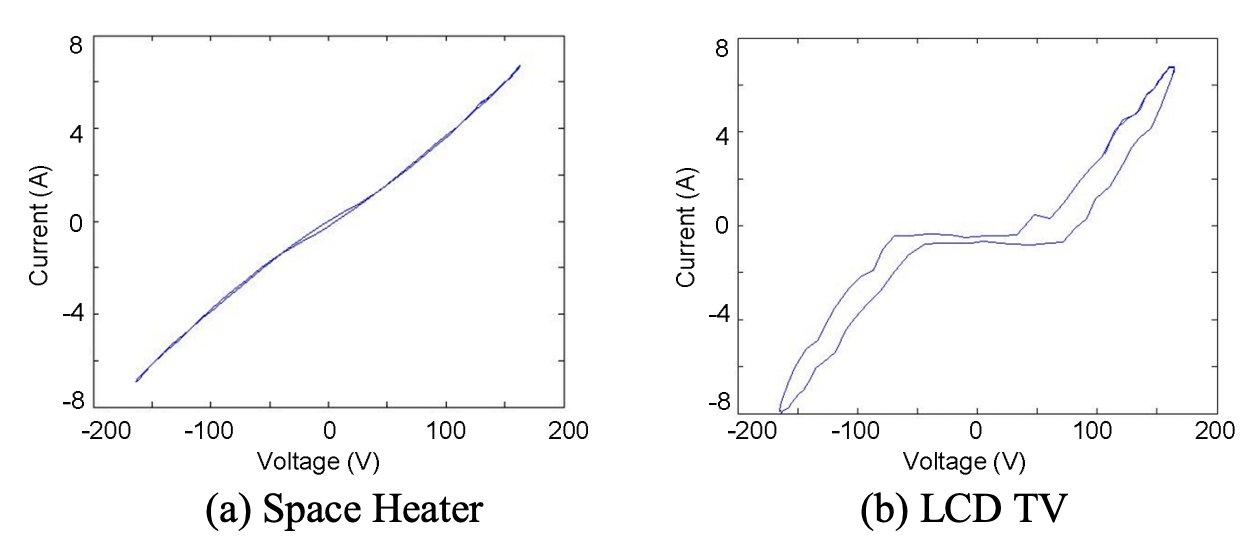
\includegraphics[scale=0.6]{figure/ivfig.png} % Includes your figure and defines the size
    \caption{V-I trajectories of a space heater and a LCD TV \cite{5618423}} % For your caption
    \label{fig:my_label} % If you want to label your figure for in-text references
\end{figure}
%=========================================================================================
\subsection{Real and Reactive Power}
The variations in real and reactive power can be used to identify the types of load \cite{97667}. First, the real power (P) and reactive power (Q) are recorded by a measurement device. Then, the values are compared with a predefined database of load power. Based on the relative positions of different loads in the complex P-Q plane, the type of the load is identified. Loads which are far from each other in the plot can be identified only using real and reactive power. The success rate for load identification of large residential loads has been shown to be greater than 80 \%.
This method fails in case of many MELs in residential buildings which consume approximately same real and reactive power, so points corresponding to them are very near to each other in the P-Q plane. So, rule-based algorithms are applied to dis-aggregate loads based on real and reactive power measurements of electric energy consumption data, along with assumptions about the customer behavior. If two or more loads have similar demand levels decision tree analysis technique is used to distinguish between them, based on the assumptions such as the time of day or the length of usage.
Plot of the real and reactive power of typical loads of residential buildings in the P-Q plane \cite{192069} Figure 2.
\newline
\textbf{Cons:}
\begin{itemize}
    \item This method is based on steady-state power consumption. Therefore, it requires waiting until the transient behavior settles down so that steady-state values can be measured.
    \item Some loads in commercial and residential buildings do not yield reliable steady-state measurements.
\end{itemize}

\begin{figure}[htpb!] % Defines figure environment
    \centering % Centers your figure
    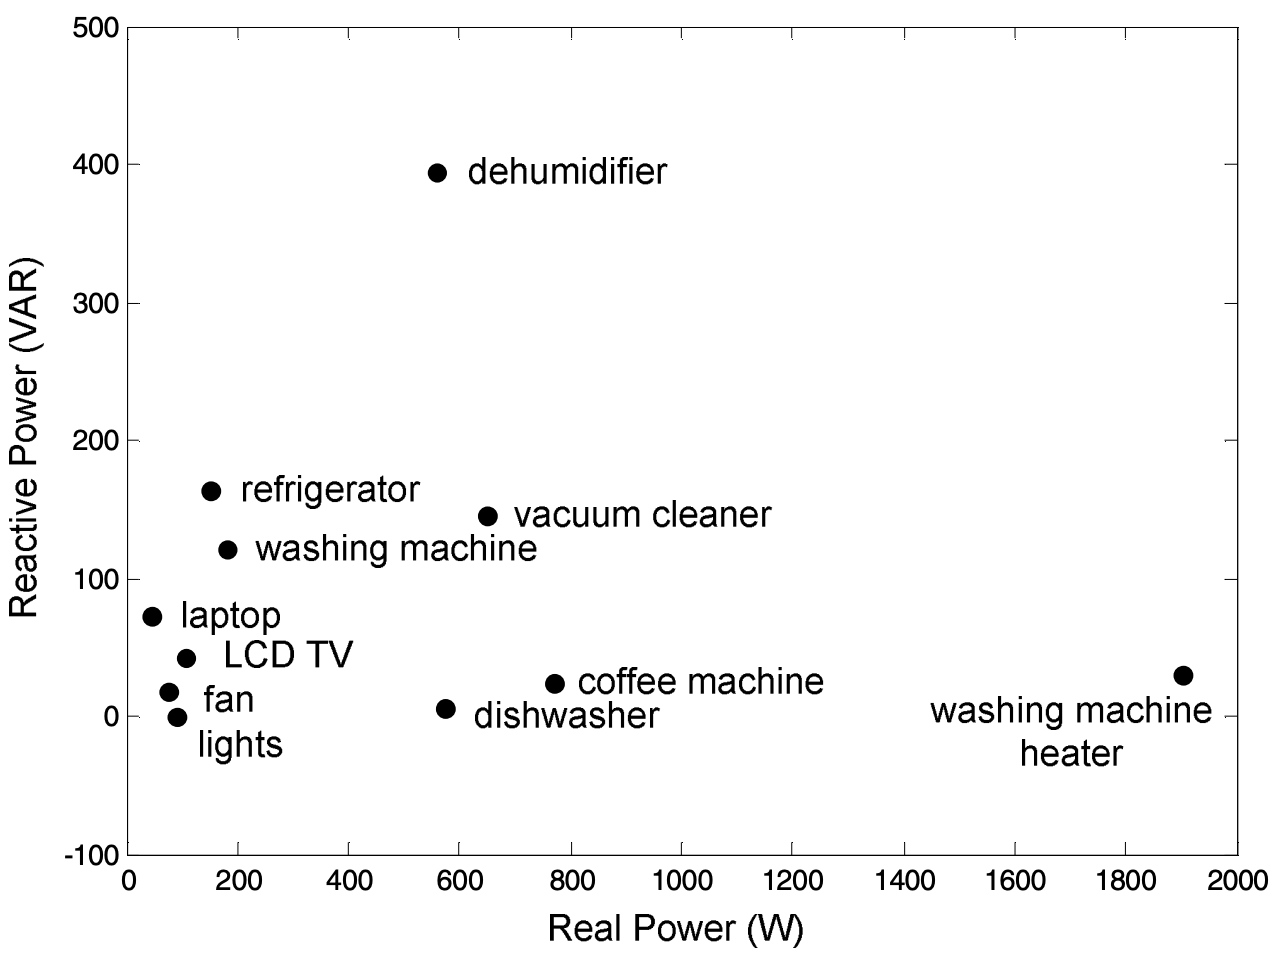
\includegraphics[scale=0.6]{figure/realvsreactfig.png} % Includes your figure and defines the size
    \caption{Real and reactive power of electric loads in residential buildings in the P-Q plane.\cite{192069}} % For your caption
    \label{fig:my_label} % If you want to label your figure for in-text references
\end{figure}
%=========================================================================================
\subsection{Eigenvalue Analysis and SVD}
In this method, time series of the current waveform are rearranged into a matrix form \cite{lam2005building}. Then SVD is applied to calculate its eigenvalues. Now different loads have different wave forms shape and hence different eigenvalues. For instance, larger loads have a higher first eigenvalue. Thus, this method can also correlate to the power consumed by the load.
\newline
\textbf{Cons:}
\begin{itemize}
    \item Since eigenvalues are defined only for square matrix, its necessary to have n cycles of data if each contains n sampled data points. So, requirement of data is higher.
    \item If sampling frequency of waveform is changed, a new matrix is obtained thus giving different eigenvalues for same load. Thus, this method is not consistent with the change of sampling rate 
\end{itemize}

%=========================================================================================
\subsection{Current Waveform Characteristic and Harmonics}
The \textbf{current waveform} and the \textbf{phase difference between the current and voltage} are good enough to describe a load\cite{Saitoh2008CurrentSB}. Peak current, average current and RMS current, displacement power factor and the total harmonic distortion in current are used as features for identification. Then \textbf{nearest neighbour technique} is applied for recognition. Other important key "steady-state signature" is the power factor. It can clearly distinguish purely resistive loads, motor-drive loads, and power electronic loads.
Non-linear loads like MELs result in harmonics. Thus, current harmonics can be used to identify these loads. To improve the identification accuracy, it can be combined together with P-Q plane methods and transient power methods for load identification.

\newline
\textbf{Cons:}
\begin{itemize}
    \item It is not feasible to compare the waveforms directly in application because of computational limitations and sensitivity issues.
\end{itemize}

%=========================================================================================
\subsection{Transient Power}
Transient behavior of a load is closely reflects the physical task that the load performs \cite{srshaw}. Hence most loads have repeating transient profiles which can help in identification of variable loads. Also, power of transient harmonics provides extra information for variable loads, which is helpful in identifying variable drive connected loads as drive startup is generally repeatable, controlled by a microprocessor. 
\newline
\textbf{Cons:}
\begin{itemize}
    \item High sampling rate and continuous monitoring are required to analyze transient power.
\end{itemize}
%=========================================================================================
\begin{figure}[htpb!] % Defines figure environment
    \centering % Centers your figure
    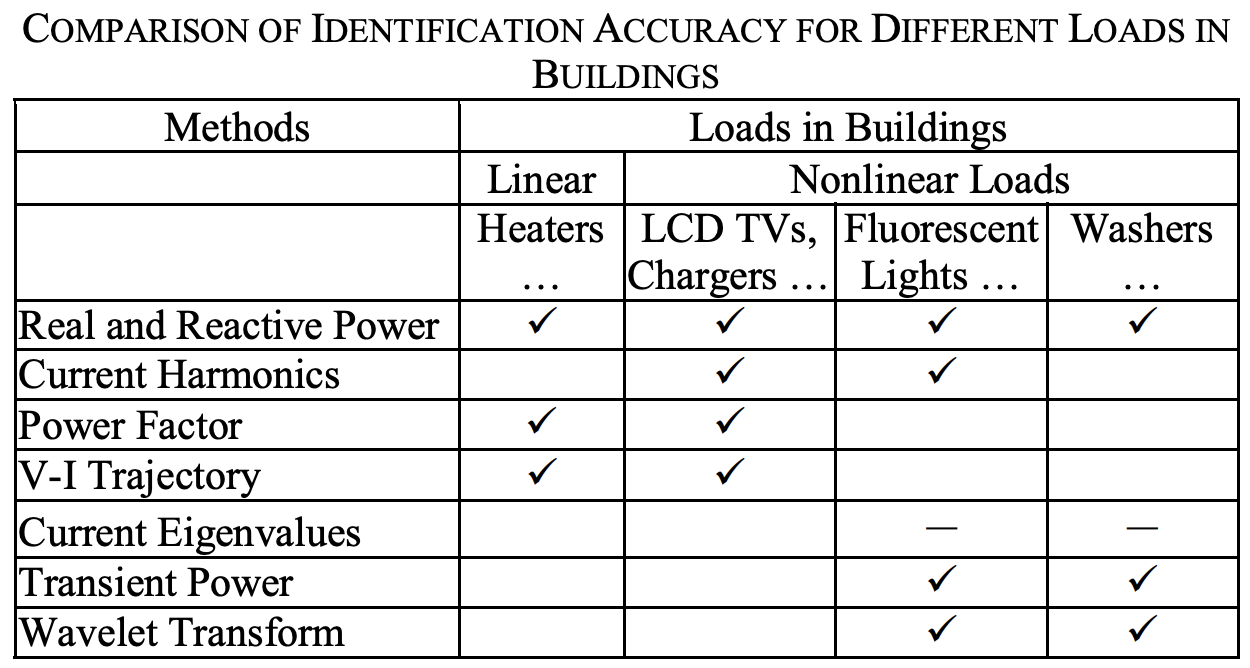
\includegraphics[scale=0.6]{figure/methodsfig.png} % Includes your figure and defines the size
    \caption{Comparison of Identification Accuracy for Different Loads in Buildings\cite{192069}} % For your caption
    \label{fig:my_label} % If you want to label your figure for in-text references
\end{figure}

%=========================================================================================
\subsection{Optimization of Identification metrics}
Here, the objective function is defined as the minimum residue while comparing the unknown loads with a set of candidates extracted from the known database, as given below \cite{97667}.

\[ min \; Obj_j = \sum_{k = 1}^{N} w_k(\hat{y}_{(kj)} - y_{(k)})^2 \]
\begin{flushleft}
$\hat{y}_{(kj)}$ = feature k extracted from the known feature-database of load j \\
$y_{(k)}$ = feature k extracted from the unknown load \\
$w_k$ = weight of feature k \\
$N$ = total number of features \\
\end{flushleft}

A one-to-one comparison with the known database is performed when the load features are extracted from a single load. The residue is computed between the unknown and the known individual load signatures. The target load is the known load with the minimum residue. The weight of a feature, $w$ helps to adjust the significance of features. \newline
When the unknown is a composite load containing more than one load's signature, the optimization method becomes more complex. Methods such as genetic algorithms \cite{Cheng2006ElectricLoadI}, integer programming, dynamic programming approaches, particle swarm optimization, fuzzy logic or multi-algorithm framework have been proposed to solve this problem.

\newline
\textbf{Cons:}
\begin{itemize}
    \item This method assumes that all features of loads are already known and it is largely based on this database whereas many loads have several operating states and they consume different level of power in different states. 
    \item For example, a TV set could be in operating, standby, and off modes. It generally consumes less power in standby mode than the operating mode, but the features are almost the same except in magnitudes. Thus, methods based on optimization method could be totally wrong in some cases.
\end{itemize}

%================================================================================

\subsection{Artificial Neural Networks}
Artificial neural networks (ANN), can be used to identify the appliance loads by training it to learn the specific features of different appliances. It is suggested in \cite{351862} to train a number of neural networks in cascade, which are then used as pattern classifiers to identify the various loads. Steady-state appliance signatures, such as fundamental frequency quantities, current, power and impedance contours and harmonic frequency current information and distortion power serve as the inputs of neural networks.
Multi-layer-perceptron (MLP), radial-basis-function (RBF), and support vector machines (SVM) are applied in \cite{950402}, \cite{1564224}. Data from Fourier analysis of the input current waveform of multiple devices are used to train the models. A comparison of performance showed that multi-layer-perceptron and SVM-based models are good to determine the presence of particular loads based on their harmonic signatures.
\newline
\textbf{Cons:}
\begin{itemize}
    \item These methods cannot visualize the high dimensional data before and after the pattern recognition process. SVM can give good accuracy using non-linear kernel, but it does not show the reason of the failure and which load is most likely to be recognized.
\end{itemize}

\section{Base Papers}
One of our base papers is \cite{barsim2018neural}.
Post segmentation of the constituent appliances from the acquired raw data, our task will be to identify these said appliances. 
\subsection{WHAT is the method and WHY utilize it}
Neural Networks have been a largely un-utilized technique in this application. Ensemble methods are used because they have been shown to give much more accurate results in applications where we expect diverse input vectors. Ensemble methods rely on the observation that the results of multiple weakly trained networks when combined appropriately, outputs a comparatively better result. There are different ensemble techniques that can be used to combine the results. These techniques differ majorly on the basis of the composition of constituent networks (homogeneous, heterogeneous). 
\subsection{Detailed Explanation}
The sampling frequency of the data-set (PLAID plug load appliance identification data-set) is 30KHz with a grid frequency of 60Hz. One of the advantages of Neural Network based techniques is one of not being reliant on extraction of features that are hard-coded.

\begin{enumerate}
    \item Using the provided sampling and grid frequencies, we extract one complete cycle from the raw I and V data. Each period will have a total of $d = f_s/f_g$ samples per period.
    \item Normalization of data on the range of $[-1,1]$. This is a standard procedure which is known to aid the learning of Neural Networks.
    \item We then construct the input vector for the Network by stacking the normalised I and V values to create a $2d\times1$ dimensional vector.
    \item We augment/expand the data by introducing phase shift of $\epsilon$ samples $d/\epsilon$ times. The advantage of this step is that it removes the need to phase align the data and makes the Network much more robust to phase variations in the input data. Neural Networks are also very data hungry algorithms and thus benefit from more data.
\end{enumerate}

\subsubsection{Ensembling}
Ensembling is a techniques which is very well known for increasing the accuracy and robustness of the Network to input data especially in the case where the learning algorithms is sensitive to changes in training set. It combines multiple small scale neural networks trained for completing small subsets of a problem to determine the solution to the bigger problem as a whole. Specifically we use the \textbf{Bootstrap Aggregation} ensembling technique.

Going by the notation of the basis paper, Given a set $\Omega = \{w_m\}_{m = 1}^M$ of M classes, for each class combination $(w_i,w_j)_{i<j}$, a binary classification neural network $\hat{\theta}_{w_i,w_j}$ is trained on the appropriately selected subset of training data(i.e. where the true class of the example is $w_i$ or $w_j$). Hence in total, we train $M \choose 2$ base models.

Finally, our base neural networks output: 
\[\hat{\theta}_{w_i,w_j}(x) = \big[ \hat{p}_{w_i,w_j}(x),\hat{p}_{w_j,w_i}(x)\big]\]

where, $\hat{p}_{w_i,w_j}(x)$ is the probability that the input data $x$ belongs to class $w_i$ over class $w_j$ in which case, the target vector for our network $\hat{\theta}_{w_i,w_j}$ becomes $[1,0]$.

Our final ensemble prediction can take two forms:\\
\textbf{Confidence Weighted Voting}
\[\hat{w}(x) = \argmax_{w_i \in \Omega} \sum_{j \neq i} \hat{p}_{w_i,w_j}(x)\]
\textbf{Un-weighted Majority Voting}
\[\hat{w}(x) = \argmax_{w_i \in \Omega} \sum_{j \neq i} \mathbbm{1} \big( \hat{p}_{w_i,w_j}(x) > \hat{p}_{w_j,w_i}(x) \big)\]

here $\mathbbm{1}$ is the indicator function to return binary output based on the parenthesized condition.

Finally, the author uses validation based early stopping to prevent over-fitting utilizing 30 \% of the train set as validation. 

\subsection{Evaluation}
The author uses the PLAID publicly available data-set with $M$ = 11. Hence a total of $M \choose 2$ base networks are trained. The dimensions of the networks are as follows: \newline
\begin{center}
2 layer fully-connected Neural Network \\
    $2d$ input neurons \\
    $30$ hidden neurons \\
    $2$ output neurons \\
\end{center}

Due to existence of transients, the last two cycles of each measurement are taken. $\epsilon$ = 10 samples expands the data-set by a factor of $d/\epsilon$ = 50. The $\tanh$ activation function is chosen for the neurons expect for the output layer which utilizes the $softmax$ function. Further, the utilize MATLAB's implementation of conjugate gradient descend. Samples from one building are separated out as the test set.


% We normalize the data [-1,1].

% Stacking the I and V sample data gives us the input vector of dimensions 2d * 1.

% Augmentation/ Expansion of the data by phase shifting the acquired cycle based on a epsilon = sliding step. This gives up d/epsilon times more data to work with. Furthermore, it removes the need to phase align the input data and makes our network more robust to signal variations.

% Details of ensembling:
% We use an ensemble of binary networks (i.e. networks with two binary outputs).
% For m classes, we’ll have mC2 networks. Each network is expected to output [1 0] or [0 1] based on what class of appliance it believes the input data belongs to.

% Let Pij be probability of class i over class j.

% Our final ensemble function can either be (eqn 7) or (eqn 8).

% The paper uses validation based early stopping as a regularization method.

\section{Results}
\begin{figure}[htpb!] % Defines figure environment
    \centering % Centers your figure
    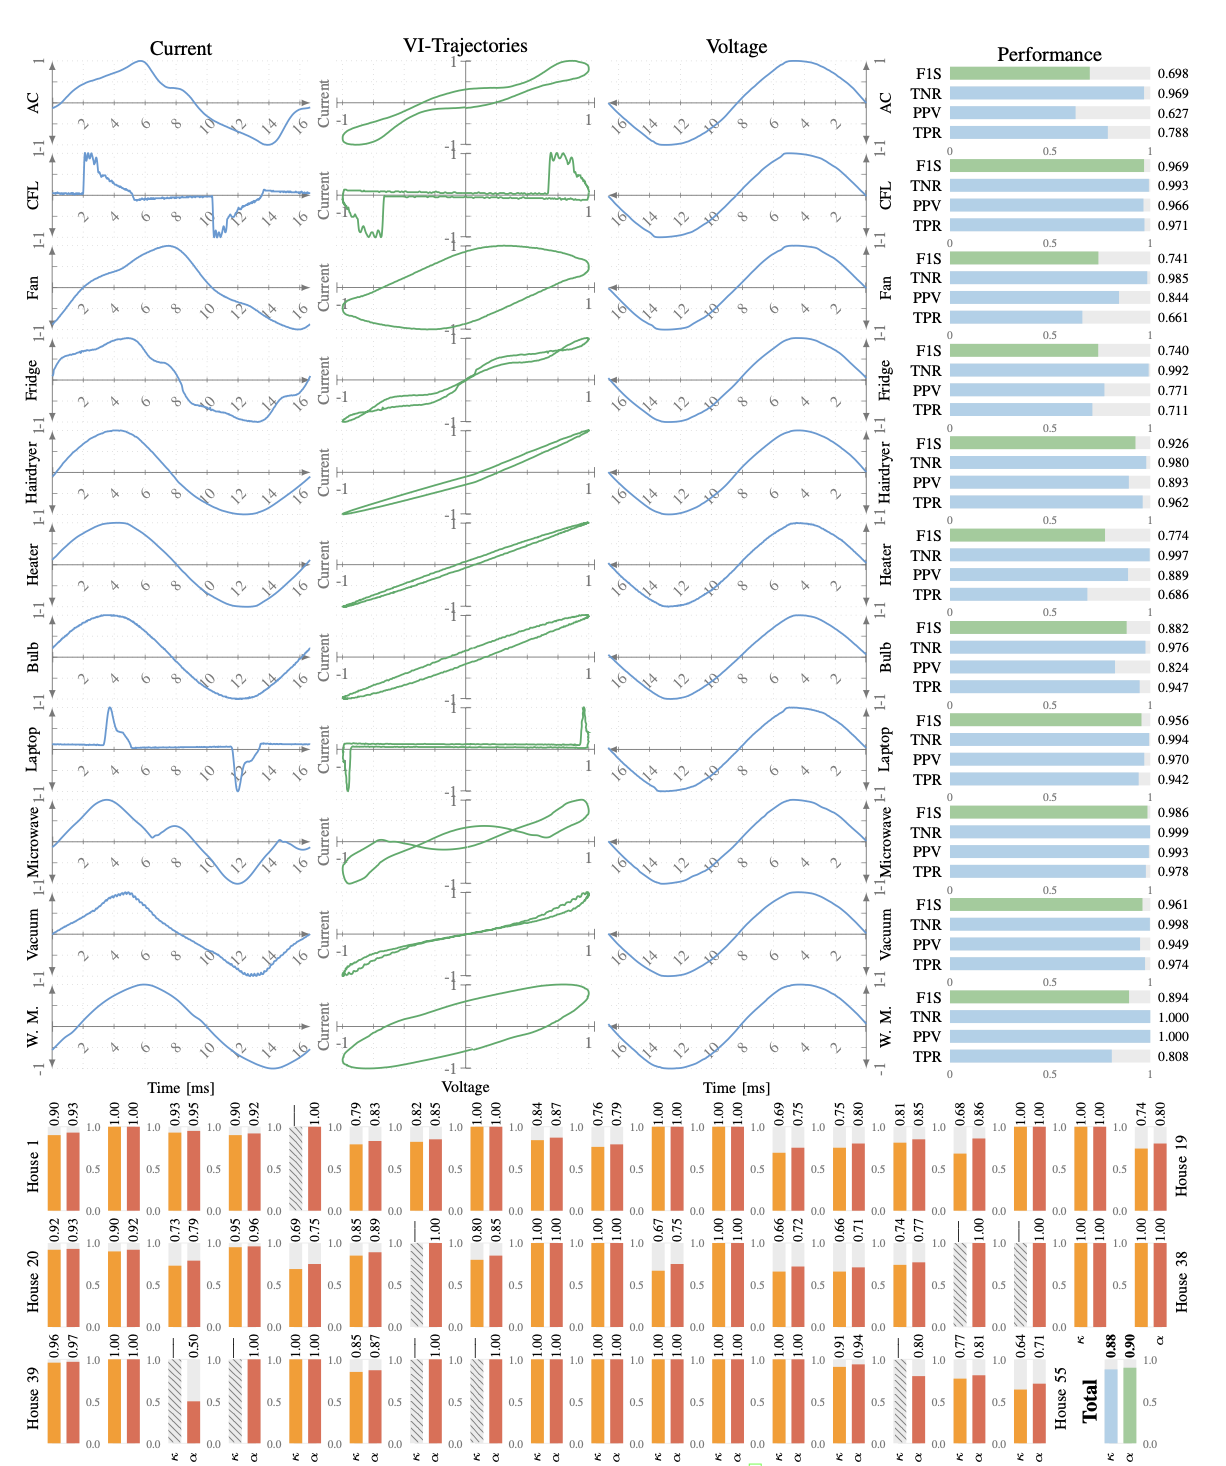
\includegraphics[scale=0.8]{figure/results.png} % Includes your figure and defines the size
    \caption{Current, voltage, and VI-trajectories of selected samples from PLAID dataset \cite{plaid} are shown to the left. The appliance categories and IDs, from top to bottom, are (1) air conditioner, 1010, (2) CFL, 20, (3) fan, 766, (4) fridge, 6, (5) hairdryer, 444, (6) heater, 716, (7) bulb, 57, (8) laptop 28, (9) microwave, 10, (10) vacuum cleaner, 730, and (11) washing machine, 488. The per-category evaluation metrics are shown to the right while the per-house metrics are in the bottom. The best evaluation results are κ = 0.882 and α = 0.897.\cite{barsim2018neural}} % For your caption
    \label{fig:my_label} % If you want to label your figure for in-text references
\end{figure}

\begin{figure}[htpb!] % Defines figure environment
    \centering % Centers your figure
    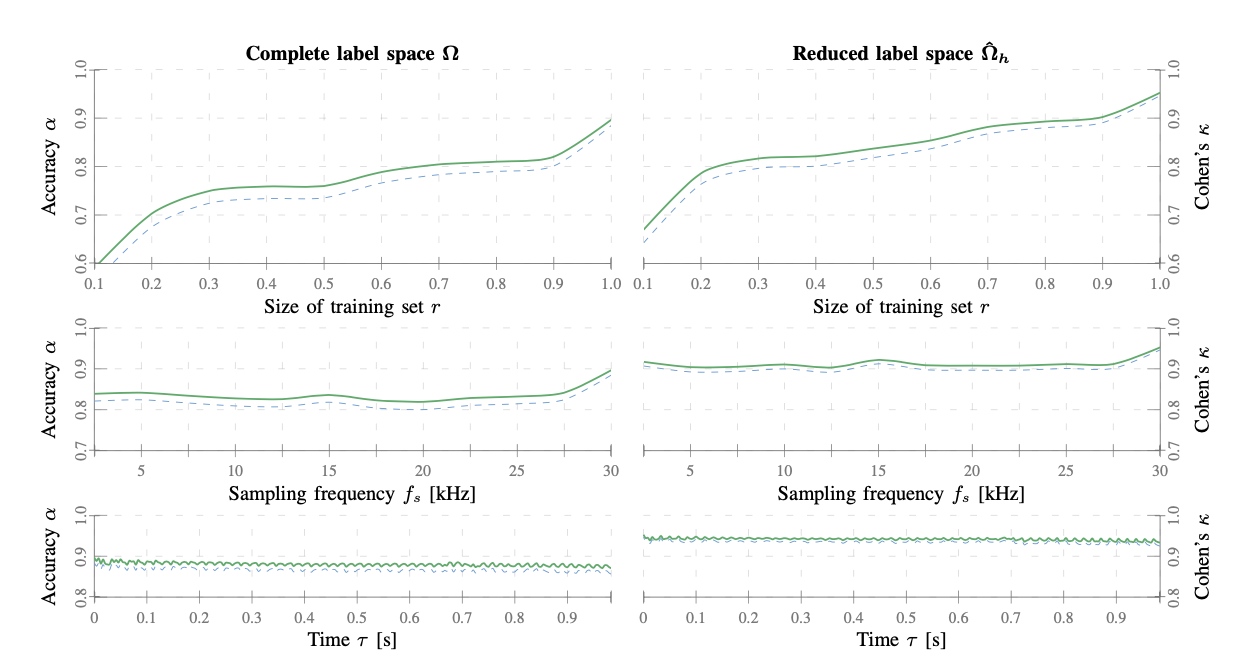
\includegraphics[scale=0.8]{figure/results2.png} % Includes your figure and defines the size
    \caption{Aggregate evaluation results as a function of (a) training set size, (b) sampling frequency, (c) time shift. On the right are the same experiments with reduced label spaces based on prior knowledge of the label space for each target household\cite{barsim2018neural}} % For your caption
    \label{fig:my_label} % If you want to label your figure for in-text references
\end{figure}

\begin{center}
    F!S = F-1 Score \\
    TPR = recall \\
    PPV = precision \\
    TNR = specificity \\
\end{center}
\begin{itemize}
    \item As we can clearly see in the experimental results shown in figure 5, Reduction in training set size to a factor $r$ has a very noticeable and drastic effect on the accuracy of the network.
    \item Although the reduction in sampling frequency has a visible effect, the model is able to maintain the accuracy above 80\% even at sampling rates lower than 5KHz. This shows that most of the extracted features are [present in the lower frequencies.
    \item We can see in the third study that introducing phase displacement has negligible effect on the accuracy of the network.
    \item Knowledge about the list of appliances of each house hold can noticeably improve the performance. However, it must be kept in mind that the availability of this information is not easy.]
\end{itemize}


\printbibliography
% \section{Introduction} % Add a section title
% \subsection{Highlighting} % Add a subsection
% \LaTeX allows you to highlight text in various ways: \textbf{bold}, \textit{italics}, with \textsc{small caps} or \texttt{as a coding font}.\footnote{ This command adds a footnote to your text.} 

% \subsection{Citing} % Add another subsection
% Citing in \LaTeX is easy. You could easier cite with the text flow like this ``Referring to \citet{collier2004greed} ...''  or at the end of the sentence \cite{collier2004greed}. You can also cite pages like this \citep[55]{collier2004greed}. If you want to add an additional note, you might want to do it this way \citep[cp.][22]{collier2004greed} or like this \citep[cp.][]{collier2004greed}.\\
% \blindtext % Adds some blintext to your text

% %----------------------------------------------------------------------------------------
% % Literature review
% %----------------------------------------------------------------------------------------

% \section{Literature review}

% \blindtext % Some blind text

% \subsection{Some subsection}
% \blindtext % Some more blind text

% \subsubsection{And a subsubsection}
% \blindtext % Even more blind text

% And here you have a list with dots and dashes:
% \begin{itemize}
%     \item Dots 
%     \item[-] or dashes?
% \end{itemize}

% and an enumerated list:

% \begin{enumerate}
%     \item With numbers...
%     \item Which is also nice \Winkey
% \end{enumerate}

% %---------------------------------------------------------------------------------
% % Theory
% %---------------------------------------------------------------------------------

% \section{Theory}

% If you want to add mathematical equations, this may be done either this way: $a +  b \neq \frac{a}{b}$. You may also add Greek letters like this: $\alpha$.\\ 

% \blindtext % Some blind text

% % Including figures
% \begin{figure}[htpb!] % Defines figure environment
%     \centering % Centers your figure
% 
\includegraphics[scale=0.8]{figure/figure.png} % Includes your figure and defines the size
%     \caption{A circle} % For your caption
%     \label{fig:my_label} % If you want to label your figure for in-text references
% \end{figure}

% \blindtext % Some blind text

% % Including tables
% %   Simple table
% \begin{table}[] % Add htpb! to make sure that table is where it should be
%     \centering
%     \begin{tabular}{c|c}
%         Saturday & Sunday \\
%         12 & 18
%     \end{tabular}
%     \caption{Overview of the weekend}% Caption for tables
%     \label{tab:weekend} % Reference for in-line referencing
% \end{table}

% %   Table with table generator
% \begin{table}[] % Add htpb! to make sure that table is where it should be
%     \centering
% \begin{tabular}{@{}lll@{}}
% \toprule
%   & A   & B \\ \midrule
% C & 100 & 2 \\
% D & 3   & 5 \\ \bottomrule
% \end{tabular}
%     \caption{Random numbers} % Caption for tables
%     \label{tab:numbers} % Reference for in-line referencing
% \end{table}

% %----------------------------------------------------------------------------------------
% % Research design
% %----------------------------------------------------------------------------------------

% \section{Research Design}

% \blindtext % Some blind text

% %----------------------------------------------------------------------------------------
% % Analysis
% %----------------------------------------------------------------------------------------

% \section{Analysis}

% \blindtext % Some blind text

% %----------------------------------------------------------------------------------------
% % Conclusion
% %----------------------------------------------------------------------------------------

% \section{Conclusion}

% \blindtext % Some blind text

% %----------------------------------------------------------------------------------------
% % Bibliography
% %----------------------------------------------------------------------------------------
% \newpage % Includes a new page

% \pagenumbering{roman} % Changes page numbering to roman page numbers
% %\bibliography{literature}

% Add the filename of your bibliography
% \bibliographystyle{apsr} % Defines your bibliography style

% % For citing, please see this sheet: http://merkel.texture.rocks/Latex/natbib.php

% %----------------------------------------------------------------------------------------
% % Appendix
% %----------------------------------------------------------------------------------------
% \newpage % Includes a new page
% \section*{Appendix} % Stars disable section numbers
% % \appendix % Uncomment if you want to add an "automatic" appendix
% \pagenumbering{Roman} % Changes page numbering to Roman page numbers

% \blindtext % Adds some blind text

% %----------------------------------------------------------------------------------------
% % Declaration
% %----------------------------------------------------------------------------------------
% \newpage % Includes a page break
% \thispagestyle{empty} % Leaves the page style empty (no page number, no header, no footer)
% \section*{Statutory Declaration} % Stars disable section numbers

% \begin{otherlanguage}{german}
% Hiermit versichere ich, dass diese Arbeit von mir pers\"{o}nlich verfasst ist und dass ich keinerlei fremde Hilfe in Anspruch genommen habe. Ebenso versichere ich, dass diese Arbeit oder Teile daraus weder von mir selbst noch von anderen als Leistungsnachweise andernorts eingereicht wurden. W\"{o}rtliche oder sinngem\"{a}{\ss}e \"{U}bernahmen aus anderen Schriften und Ver\"{o}ffentlichungen in gedruckter oder elektronischer Form sind gekennzeichnet. S\"{a}mtliche Sekund\"{a}rliteratur und sonstige Quellen sind nachgewiesen und in der Bibliographie aufgef\"{u}hrt. Das Gleiche gilt f\"{u}r graphische Darstellungen und Bilder sowie f\"{u}r alle Internet-Quellen. Ich bin ferner damit einverstanden, dass meine Arbeit zum Zwecke eines Plagiatsabgleichs in elektronischer Form anonymisiert versendet und gespeichert werden kann. Mir ist bekannt, dass von der Korrektur der Arbeit abgesehen und die Pr\"{u}fungsleistung mit nicht ausreichend bewertet werden kann, wenn die Erkl\"{a}rung nicht erteilt wird.
% \end{otherlanguage}

% \vspace*{1in} % Adds extra space between two paragraphs

% \noindent I hereby declare that the paper presented is my own work and that I have not called upon the help of a third party. In addition, I affirm that neither I nor anybody else has submitted this paper or parts of it to obtain credits elsewhere before. I have clearly marked and acknowledged all quotations or references that have been taken from the works of others. All secondary literature and other sources are marked and listed in the bibliography. The same applies to all charts, diagrams and illustrations as well as to all Internet resources. Moreover, I consent to my paper being electronically stored and sent anonymously in order to be checked for plagiarism. I am aware that the paper cannot be evaluated and may be graded ``failed'' (``nicht ausreichend'') if the declaration is not made.\\

% %\vspace*{1in} % Adds extra space

% % Add field for signature, date, and place
% \hfill \signature{} 


%---------------------------------------------------------------------------------

\end{document}
